% Ubah judul dan label berikut sesuai dengan yang diinginkan.
\section{Design and Implementation}
\label{sec:designandimplementation}

% Ubah paragraf-paragraf pada bagian ini sesuai dengan yang diinginkan.
This research is explaining about the implementation one of the branch of deep learning studies with the aim to automatically detect Indonesian hoax news by leveraging BERT method. This detection method is trained by using a combination of dataset from \url{https://data.mendeley.com/datasets/p3hfgr5j3m/1} and dataset that we made ourself for this paper alone by using web crawling technology. Picture \ref{fig:metodologi} is the outline of this research in a nutshell.

\begin{figure} [h]
    \centering
    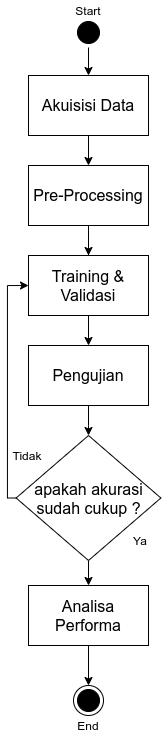
\includegraphics[width=0.3\columnwidth]{gambar/metodologi_vertical.png}
    \caption{This research method in a nutshell.}
    \label{fig:metodologi}
\end{figure}

\subsection{Material and Tools Specification}

The dataset that is being used in this research is a dataset originated from \url{https://data.mendeley.com/datasets/p3hfgr5j3m/1} coupled with our own made dataset in which we have create it using web crawling technology. Both of these dataset combined, is resulting in total of 1621 data with the exact details can be seen at table \ref{tab:dataset}. Meanwhile, table \ref{tab:dataset_mendeley} is the starting point of our dataset which we gotten from \url{https://data.mendeley.com/datasets/p3hfgr5j3m/1} alone.

Each of these dataset is containing the content of the news along with its label which can be either "Valid" or "Hoaks". We took the news from accredited and verified news sources for the valid news, while on the other side, we took all of the hoax news mostly from \url{https://turnbackhoax.id}, a website that contains the list of user reported hoax news from many sources.

\begin{table}[h]
    \caption{Total of news from \url{data.mendeley.com}}
    \label{tab:dataset_mendeley}
    \centering
    \begin{tabular}{ | l | l | }
        \hline
        \textbf{Label} & \textbf{Total Data} \\ \hline
        \textit{Hoaks} & 228                 \\ \hline
        \textit{Valid} & 372                 \\ \hline
        \textbf{Total} & \textbf{600}        \\ \hline
    \end{tabular}
\end{table}

\begin{table}[h]
    \caption{Total of training dataset}
    \label{tab:dataset}
    \centering
    \begin{tabular}{ | l | l | }
        \hline
        \textbf{Label} & \textbf{Total Data} \\ \hline
        \textit{Hoaks} & 885                 \\ \hline
        \textit{Valid} & 736                 \\ \hline
        \textbf{Total} & \textbf{1621}       \\ \hline
    \end{tabular}
\end{table}


\begin{table}[h]
    \caption{Dataset Sample}
    \label{tab:contoh_dataset}
    \centering
    \begin{tabular}{ | p{.8\linewidth} | l | }
        \hline
        \textbf{news}                                                                                                                                                                                                                     & \textbf{tagging} \\ \hline
        Wakil Gubernur DKI Jakarta Sandiaga Uno menargetkan pengerjaan tahap awal Stadion BMW dilakukan pada Oktober. Stadion ini diperuntukkan bagi klub Persija....                                                                     & Valid            \\ \hline
        "Komisi II bersama KPU dan Bawaslu masih membahas ketentuan wajib cuti bagi petahana presiden yang maju Pilpres 2019. Mekanisme pengambilan.....                                                                                  & Valid            \\ \hline
        Jaksa penuntut Ulumum (JPU) pada Komisi Pemberantasan Korupsi (KPK) mencecar Pejabat Pembuat Komitmen (PPK) reguler pada Direktorat Perlindungan Sosial Korban Bencana Sosial Kemensos Victorious Saut Hamonangan Siahaan soal... & Valid            \\ \hline
        “Halo Kak! Aku Winda Dari Team Giveaway BAIM WONG Anda Memenangkan Hadiah Uang 100Jt dari kami info klik: https://wa.me/+6285796306857”                                                                                           & Hoax             \\ \hline
        “Apa yang terjadi dengan hewan dalam penelitian?   Teknologi ini telah dicoba pada hewan, dan pada hewan penelitian yang dilakukan, semua hewan mati , tidak langsung dari suntikan...                                            & Hoax             \\ \hline
        “Kadrun istilah dr PKI alias KOMUNIS ditujukan buat islam. Kl mau jd komunis pake aja istilah kadrun buat umat islam. Auto lsg Komunis”                                                                                           & Hoax             \\ \hline
    \end{tabular}
\end{table}

\subsection{Akuisisi Data}

Because the dataset that we get from \url{https://data.mendeley.com/datasets/p3hfgr5j3m/1} feel severely lacking for our purpose because it only consist of 600 data, and because there are no web crawling which outputting its result into a convenient CSV file from Indonesian news sites, we took on our hand a task to create a webcrawling program to take news content from many Indonesian news sites, those sites included but not limited to \url{liputan6.com}, \url{detik.com}, \url{tempo.com} and others. As all of those sites is rightfully accredited and verified by the government, it is used for our valid news dataset. Our hoax news site however, only has one source from \url{turnbackhoax.id}, this is mainly because said site has quite an active forum behind it in which lots of people can report their finding of hoax text, seen and checked by lots of other people, before lastly, will be uploaded to the \url{turnbackhoax.id} site. But, the biggest factor in choosing that site compare to others is mainly because \url{turnbackhoax.id} wrote the original hoaks text in their website, this coupled with the fact that their website has some kind of structure into it has shorten our task significantly. For this research, the webcrawling process has took news from varied dates, ranging from April 2018 as the oldest to April 2021.

\begin{figure} [h]
    \centering
    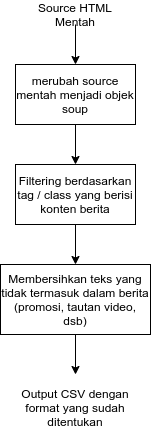
\includegraphics[width=0.35\linewidth]{gambar/webcrawl_long.png}
    \caption{Garis besar alur program \textit{web crawl}.}
    \label{fig:webcrawl_method}
\end{figure}

Picture \ref{fig:webcrawl_method} is the outline flow of the webcrawling program. Starting with inputting raw HTML code into the program, changing said code into an easier-to-process objects, get the news teks and do some post-cleaning on the text, lastly, create a .CSV file to store all of the obtained news text with the appropriate format.

\begin{lstlisting}[
    language=HTML, 
    caption={Penggalan Kode Sumber HTML \url{detik.com}.},
    label={lst:source_detik}
]

...
<div class="detail__body itp_bodycontent_wrapper">
<div class="detail__body-text itp_bodycontent">

<strong>Jakarta</strong> - Koalisi <a href="https://
detik.com/tag/jokowi" target="_blank">Jokowi</a> 
sedang menyusun visi-misi jagoannya. Setelah 
menerima masukan dari <a href="https://detik.com/
tag/muhammadiyah" target="_blank"> Muhammadiyah</a>,
 ... 
Dan kita pun membuka diri untuk menerima 
masukan untuk penyempurnaan," imbuhnya.<br><br><!--
s:parallaxindetail--><div class="clearfix"></div><style>
...

\end{lstlisting}

Firstly, we need to determine tag or class of the HTML code for our first filter. If we look into listing \ref{lst:source_detik} as a reference, we can see \texttt{detail\_\_body\-text} class is the one that containing our desired news text. We filtered that class by inputting the class name into the appropriate parameter.

More often than not, our filtering result will contain some garbage or unrelated teks resulting in the need to refine it further by post-clean it after the filter process. Usually, those teks is writer or editorial notes, ad, or related news links which we don't need at all.

Finally, is outputting all of the acquired news teks as a .CSV. There are no particular reason on the article of why we chose CSV format compared to other famous format unless CSV format is easier to use in our training program and because it is an open format that can be open by nearly any spreadsheet program.

As the general interface and improving user experience for our webcrawling software, we use a .json format file to configure what news sources that we want to get, how much is it, and when is it. All of those configuration will be processed by the program and the program will take the news in accordance with said configuration.
